\chapter{Firebase}                %crea il capitolo
%%%%%%%%%%%%%%%%%%%%%%%%%%%%%%%%%%%%%%%%%imposta l'intestazione di pagina
\lhead[\fancyplain{}{\bfseries\thepage}]{\fancyplain{}{\bfseries\rightmark}}
\pagenumbering{arabic}                  %mette i numeri arabi
\section{Storia}                 %crea la sezione


Firebase \'e una piattaforma Mobile backend as a service (MBaaS) che consente
di interfacciare applicazioni mobili e web app ad un cloud backend, fornendo allo sviluppatore servizi utili per la gestione degli utenti, storage, notifiche push e altri strumenti di analisi e sviluppo.\\
Questo tipo di modello \'e relativamente recente poich\'e si basa sul cloud computing, fornendo uno servizio globale e uniforme per connettere client differenti con la sincronizzazione dei dati in tempo reale.\\
Lo sviluppo di Firebase inizi\'o dall'omonima azienda che nel 2011 svilupp\'o la piattaforma con l'idea di fornire un servizio in grado di sincronizzare dati in tempo reale, successivamente ricevett\'e grande interessa da parte di Google che nel 2014 acquist\'o\footnote{https://techcrunch.com/2014/10/21/google-acquires-firebase-to-help-developers-build-better-realtime-apps/} Firebase e altre startup simili, integrandole con i suoi servizi Google Cloud Platform.


%https://gigaom.com/2013/06/20/firebase-gets-5-6m-to-launch-its-paid-product-and-fire-up-its-base/
% \begin{figure}[!hb]
%   \centering
%   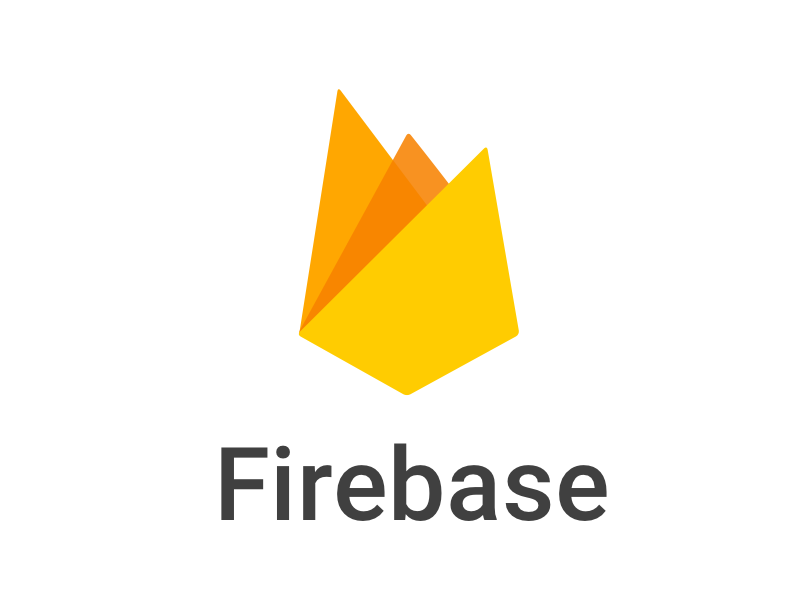
\includegraphics[width=0.25\textwidth]{immagini/firebase.png}
%   \caption{Firebase logo.}
%   \label{fig:firebase logo}
% \end{figure}




\section{Servizi}                 %crea la sezione
%https://firebase.google.com/docs/
Firebase offre diversi servizi, mettendo a disposizione anche SDK (software development kit ) e API ( Application programming interface) multipiattaforma ( Android, Ios, JavaScript, C++ e Unity) per interagire con essi.\\
I servizi offerti da Firebase sono circa 20, realizzati per facilitare lo sviluppo e la gestione del backend, permettendo ad uno sviluppatore di concentrarsi solamente sulla parte client.\\
Tra i vari servizi forniti quelli pi\'u utili nell' ambito dello sviluppo software sono:


\begin{itemize}                         %crea un elenco puntato
\item \textbf{Firebase Cloud Messaging}: Soluzione cross-platform per la gestione di notifiche push su Android iOS e Web

\item \textbf{Firebase Auth}: Servizio per la gestione degli utenti con il supporto del social login per Facebook, Github, Twitter, Google

\item \textbf{Realtime Database}: Database noSQL, con il supporto della sincronizzazione in real teim dei dati fra diversi client in diversi linguaggi di programmazione

\item \textbf{Firebase Storage}: Servizio che offre trasferimento e hosting sicuro dei file

\item \textbf{Firebase Hosting}: Web hosting che fornisce file utilizzando CDN (content delivery network) e HTTP Secure (HTTPS)


\item \textbf{Cloud Functions}: Servizio che permette di scrivere script JavaScript eseguiti ogni volta che vi \'e un cambianeto nel database Firestore/Real Time Database

\item \textbf{Firestore Database}: Database noSQl basato su documenti, con accesso ai dati offilne scalabile e con il supporto della sincronizzazione in real time
\end{itemize}

%https://firebase.google.com/products/


%https://firebase.google.com/docs/database/rtdb-vs-firestore
\section{Database}                 %crea la sezione
Google offre due differenti database con supporto della sincronizzazone dei dati in tempo reale:

\begin{itemize}
  \item \textbf{RealTime Database}
  \item \textbf{Cloud Firestore}
\end{itemize}


\textbf{RealTime Database} \'e un cloud database NoSQL che memorizza i dati in un unico file JSON. Il database risultante risulta avere una struttura ad albero con un unica radice, la struttura \'e senza schema e pu\'o quindi cambiare nel tempo.\\
Utilizzando l'SDK del RealTime Database i dati vengono mantenuti localmente, e anche quando sono offline, gli eventi in tempo reale continuano a incendiarsi, dando all' utente finale un' esperienza reattiva.\\ Quando il dispositivo riacquista la connessione, il Realtime Database sincronizza le modifiche dei dati locali con gli aggiornamenti remoti che si sono verificati mentre il client era offline, unendo automaticamente eventuali conflitti.


\textbf{Cloud Firestore} \'e un cloud database NoSQL basato sulla memorizzazione dei dati sottoforma di documenti e collezzioni di documenti, anche la sua struttura \'e senza schema e pu\'o quindi cambiare nel tempo.\\
Il modello di memorizzazione dei dati \'e basato sui documenti che possono contenere dati come stringhe e numeri, oggetti complessi e annidati.\\
Questi documenti sono archiviati in raccolte, che sono collezzioni per i documenti utilizzate per organizzare i dati e creare query.\\
\'E inoltre possibile creare subcollezioni all'interno dei documenti e creare strutture gerarchiche di dati che scalano man mano che il database cresce.\\
Gli unici limiti inposti da Firestore sono la dimensione di un singolo documento che \'e di 1 MiB (1,048,576 bytes) e un massimo di 100 collezzioni annidate.\\
Il database Firestore mantiene i dati aggiornati attraverso una buona comunicazione client-server, i client attraverso l'utilizzo delle librerie SDK  e di listener offrono una sincronizzazione in tempo reale del dati.\\
L'aggiunta di listener oltre a informare il client su modifiche effettuate nel database, permette di memorizzare le richieste effettuate in precedenza e mantenere una copia delle risposte del server nella cache, offrendo quindi un supporto offline dei dati.\\

I tipi di dato messi a disposizione da Firestore sono:

\begin{table}[h]
\begin{center}
\begin{tabular}{|p{3cm}|p{10cm}|}
    \hline
\textbf{Tipo} & \textbf{Descrizione} \\ \hline
Array & non pu\'o contenere un altro valore array. \\ \hline
Boolean & falso, vero  \\ \hline
Date & Memorizzato in formato timestamp \\ \hline
Float & precisione numerica a 64 bit \\ \hline
Geo Point & Punto geografico contentente latitudine e longitudine \\ \hline
Integer & Intero Numerico a 64 bit \\ \hline
Map & Rappresenta un oggetto  \\ \hline
Null & valore nullo \\ \hline
Reference & Riferimento ad un'altro documento nel database  \\ \hline
String & Stringa di testo codificata in UTF-8.\\
\hline
\end{tabular}
\caption[Dati Firestore ]{Data type firestore}\label{tab:Firestore Dati}
\end{center}
\end{table}

L' interrogazione del database Firestore attraverso query risulta essere molto espressivo ed efficiente. \'E possibile creare query per filtrare solo alcuni dati all'interno di un documento o filtrare collezzioni, con la caratteristiche basilari delle interrogazioni: l'ordinamento, il filtraggio e limiti sui risultati di una query. Si possono filtrare anche sottocampi di un oggetto map, ma non \'e possibile filtrare o ordinare un elemento di tipo Reference che serve solo ad indicare il riferimento di un documento all'interno del database.\\
Cloud Firestore offre un SDK con una buona integrazione per dispositivi mobili Android, iOS e web apps, ma permette l'utilizzo dei servizi anche offrndo SDK aggiuntive per altri linguaggi di programmazione come: NodeJS, Java, Python, e GO.\\


Ricapitolando, possiamo definire Firestore come una nuova versione di Firebase RealTime con una miglior struttura interna di memorizzazione dei dati e una espressivit\'a della query maggiore.

\begin{table}[h]
\begin{center}

\begin{tabular}{|p{7cm}|p{7cm}|}
    \hline
    \textbf{RealTime Firebase} & \textbf{Firestore} \\ \hline
    Memorizza i dati in un unico file JSON & Memorizza i dati in collezzioni contententi documenti \\ \hline
    Supporto per i dati offline su Android e iOS & Supporto per i dati offline su Android, iOS e Web \\ \hline
    Depp Query con ordinamento e condizioni sui dati limitate & Query con ordinamento, condizioni sui dati, indicizzazione, alte performance \\ \hline
    Memorizzazione di dati come singole operazioni. & Memorizzazione e transizioni sui dati atomiche.\\ \hline
    Validazione dei dati manuale, e settaggio manuale di regole di protezione sui dati &  Validazione dei dati automatica, e regole di protezione sui dati manuali\\
\hline
\end{tabular}
\caption[Firebase vs Firestore ]{Cofronto dei due database Firebase}\label{tab:FirestorevSFirebase}
\end{center}
\end{table}



\subsection{Database Rules}                 %crea la sezione
Firebase offre per i suoi due database la possibilit\'a di inserire delle restrizioni e regole di sicurezza per l'accesso, chiamate Database Rules.\\
Le Database Rules determinano chi ha accesso in lettura e scrittura al database o a collezzioni di dati all'interno del database, queste regole sono presenti sui server Firebase e vengono applicate automaticamente ad ogni modifica. \\
Ogni richiesta di lettura e scrittura di dati nel database sar\'a completata solo se le regole lo consentono.\\
Entrambi i database: Real time e Firestore supportano le Database Rules, le differenze fra i due servizi riguardano il metodo con cui vengono scritte le regole e il tipo di controlli che \'e possibile effetuare.\\
Firebase permette di sccrivere le regole utilizzando un file in formato JSON in cui vengono definite le regole in base alla collezzione in cui si trovano i dati, alla validazione dei dati o in base all'utente loggato su Firebase Auth.\\
Le regole applicate al database RealTime hanno una sintassi simile a JavaScript e mettono a disposizione del programmatore quattro tipi di controlli:

\begin{table}[h]
\begin{center}
\begin{tabular}{|p{2cm}|p{12cm}|}
    \hline
    {\textbf{Tipo}} & {\textbf{Descrizione}} \\ \hline
    .read & Descrive se e quando i dati possono essere letti dagli utenti.\\ \hline
   .write & Descrive se e quando i dati possono essere scritti dagli utenti\\ \hline
     .validate & Definisce l'aspetto di un valore formattato correttamente, se ha attributi figli e il tipo di dato\\ \hline
    .indexOn & Specifica una collezzione da indicizzare per supportare l' ordine e l' interrogazione\\ \hline
\end{tabular}
\caption[Firbase Rules ]{Firebase Rules}\label{tab:Firebase Rules}
\end{center}
\end{table}

La stesura delle regole per il database RealTime viene memorizzata in formato JSON sui server Firebase, un esempio di alcune regole applicate su un database \'e il seguente:


\begin{lstlisting}[language=javascript,caption={Firebase Rules esempio }]
{
  "rules": {
    "users": {
      "$uid": {
        ".write": "$uid === auth.uid"
      }
    },
    "collection2": {
     ".validate": "newData.isString() && newData.val().length < 100"
   }
  }
}
\end{lstlisting}




Le regole di sicurezza del database Firestore sono simili a quelle del RealTime Database ma prevedono un controllo degli accessi e della convalida dei dati in un formato pi\'u semplice ma espressivo.\\
Tutte le regole di sicurezza Cloud Firestore sono costituite da dichiarazioni di corrispondenza chiamate "match" che identificano i documenti nel database e consentono la creazione di espressioni che controllano l' accesso a tali documenti.\\
Oltre alle regole di scrittura, letttura, condalidazione \'e possibile creare funzioni ausiliarie per semplificare e rendere pi\'u intuitivo la scritture delle regole.\\
Un esempio di scrittura di alcune regole su un database Firestore \'e il seguente:

\begin{lstlisting}[language=javascript,caption={Firestore Rules}]
service cloud.firestore {
  match /databases/{database}/documents {
    function signedInOrPublic() {
      return request.auth.uid != null || resource.data.visibility == 'public';
   }
  match /cities/{city} {
      allow read: if request.auth.uid != null;
      allow create: if exists(/databases/$(database)/documents/users/$(request.auth.uid))
  }
 }
}
\end{lstlisting}



\section{Cloud Functions}                 %crea la sezione

Le Cloud Functions consentono di eseguire automaticamente il codice backend in risposta a modifiche effettuate nel database Firestore o RealTime.\\
I linguaggi utilizzati per scrivere le Cloud Functions sono JavaScript e TypeScript, una volta scritta una funzione essa viene memorizzata e gestita dai server Google e man mano che il carico aumenta o diminuisce, Google scala automaticamente il numero di istanze di server virtuali necessari per eseguire le funzioni.


Il ciclo di vita di una funzione \'e il seguente:
\begin{itemize}
  \item Lo sviluppatore scrive il codice per una nuova funzione, selezionando un provider di eventi (Realtime Database, Firestore) e definisce le condizioni in cui la funzione deve essere eseguita
  \item Lo sviluppatore tramite un tool a linea di comanda invia la funzione sui server di Firebase
  \item Quando il provider dell' evento genera un evento che corrisponde alle condizioni della funzione, il codice viene eseguito
  \item Se sono presenti pi\'u eventi da gestire contemporaneamente, Google creer\'a pi\'u instanze per gestire il lavoro pi\'u velocemente
  \item Quando lo sviluppatore aggiorna la funzione distribuendo il codice aggiornato, tutte le istanze per la vecchia versione vengono ripulite e sostituite da nuove istanze
  \item Quando uno sviluppatore cancella la funzione, tutte le istanze vengono ripulite e la connessione tra la funzione e il provider dell' evento viene rimossa
\end{itemize}


\newpage              % ends first column but not page
Cloud Functions mette a disposizione 4 tipi di controllo sui dati del database:

\begin{table}[h!]
\begin{tabular}{|p{2cm}|p{12cm}|}
    \hline
    \textbf{Evento} & \textbf{Trigger} \\ \hline
    onCreate &  Attivato quando si scrive un documento per la prima volta.\\ \hline
    onUpdate &  Attivato quando esiste gi\'a un documento e se ne modifica un valore.\\ \hline
    onDelete &  Attivato quando un documento con dati viene eliminato.\\ \hline
    onWrite & Attivato quando si attiva onCreate, onUpdate o onDelete.\\ \hline

\end{tabular}
\caption[Firestore Rules ]{Firestore Rules}\label{tab:Firestore Rules}
\end{table}


La scrittura di una funzione viene effettuata con la scrittura di funzioni JavaScript o TypeScript, indicando il documento o collezzione sui cui si vuole fare riferimento seguito dal tipo di evento:



\begin{lstlisting}[language=javascript,caption={Cloud functions esempio 1 }]
exports.myFunctionName = functions.firestore.document('users/koci').onWrite((event) => {
    ...
  });
exports.modifyUser = functions.firestore.document('users/{userID}').onWrite(event => {
    //  documento sottoforma di oggetto
    var document = event.data.data();
    // documento precedente alla modificarlo
    var oldDocument = event.data.previous.data();
    ...
});
\end{lstlisting}


\newpage              % ends first column but not page
\subsection{Esempi di utilizzo}
Le cloud functions possono essere utilizzati anche interagendo con gli altri servizi Firebase, un esempio di integrazione tipico potrebbe essere quello di creare un'anteprima di un immagine e salvarla su Firebase storage:

\begin{figure}[!hb]

  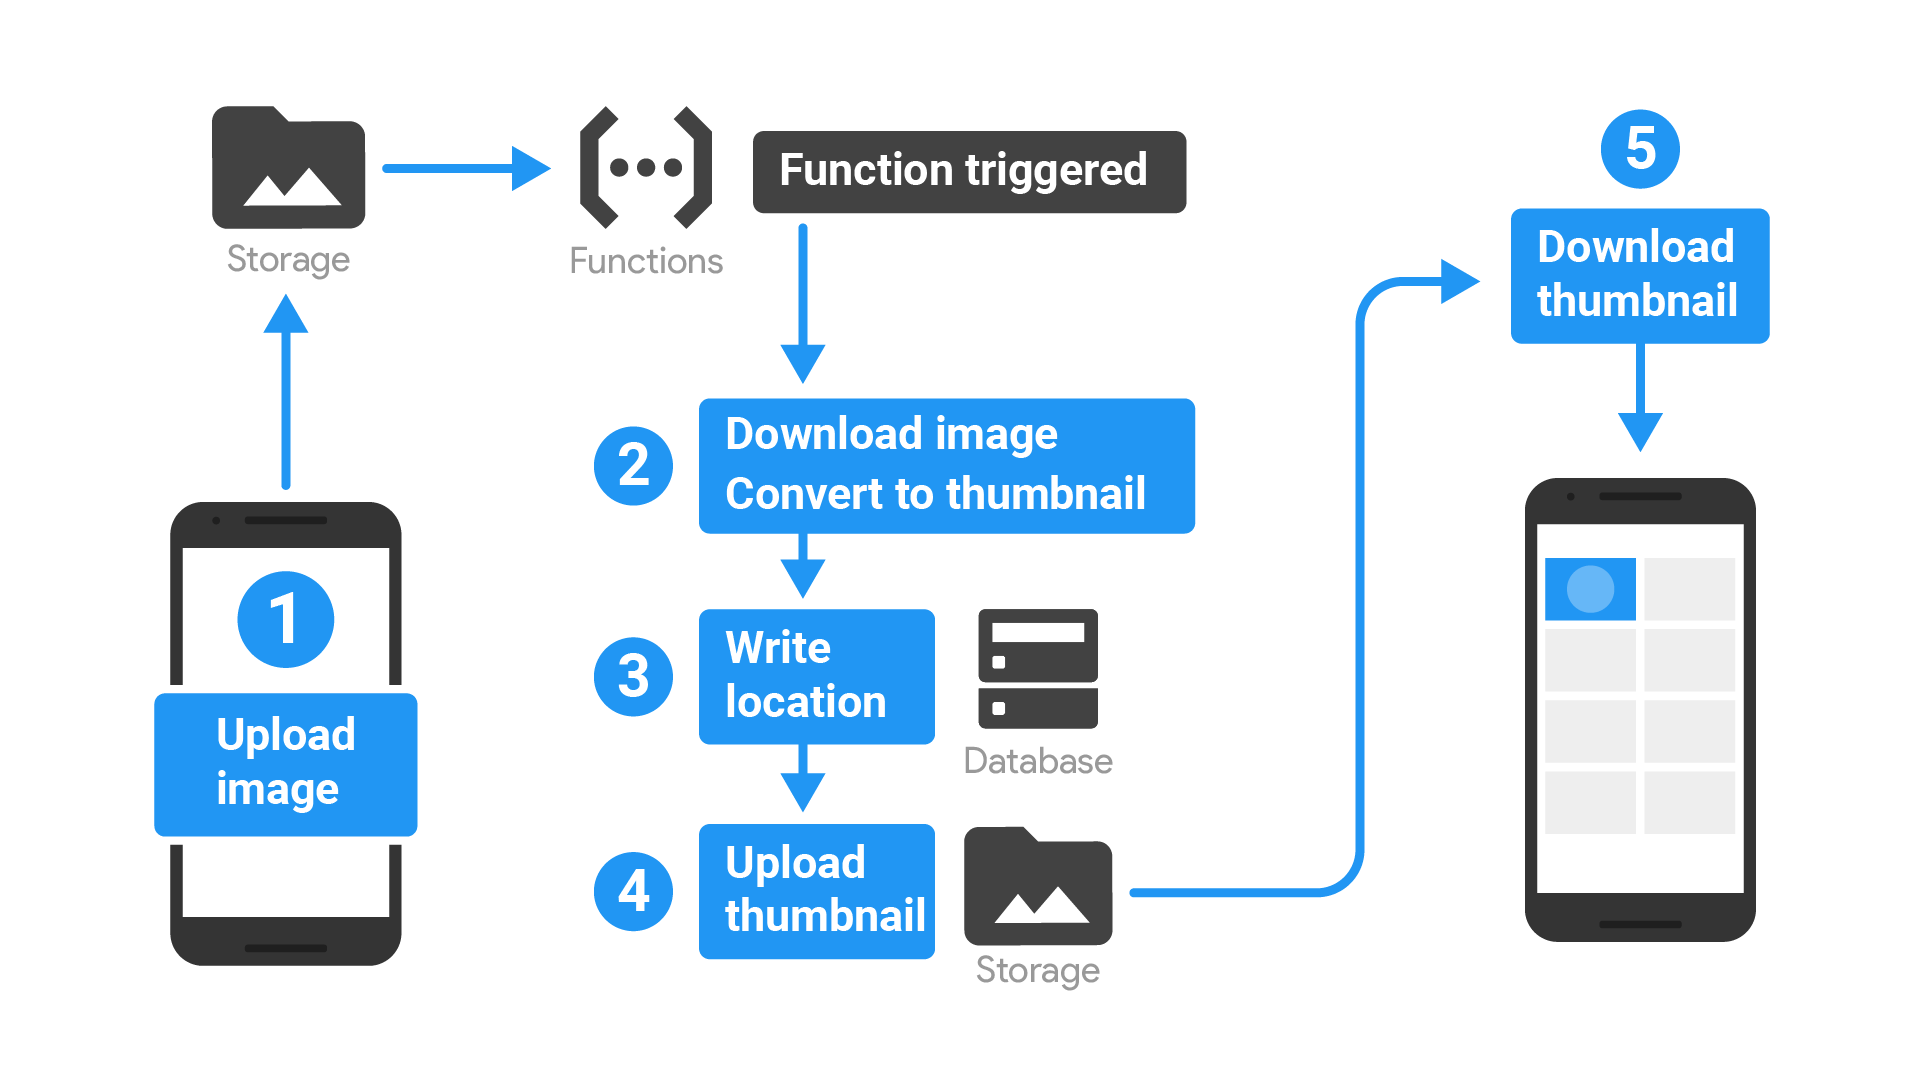
\includegraphics[width=0.8\textwidth]{immagini/functions_ex1.png}
  \caption{Firebase Storage e Cloud Functions esempio 1}
  \label{fig:Firebase Storage e Cloud Functions esempio 1}
\end{figure}

In questo esempio un funzione si attiva quando un immagine viene caricata in sullo storage firebase, la funzione scarica l'immagine e ne crea una versione miniaturizzata, in seguito scrive il riferimento della miniatura sul database, in modo che un'applicazione client possa trovarla e utilizzarla.\\

Un'altro esempio \'e l'utilizzo delle cloud functions per effettuare controlli su un tipo di linguaggio inappropriato all'interno di una chat,forum o commento:\\

\begin{figure}[h!]
  \centering
  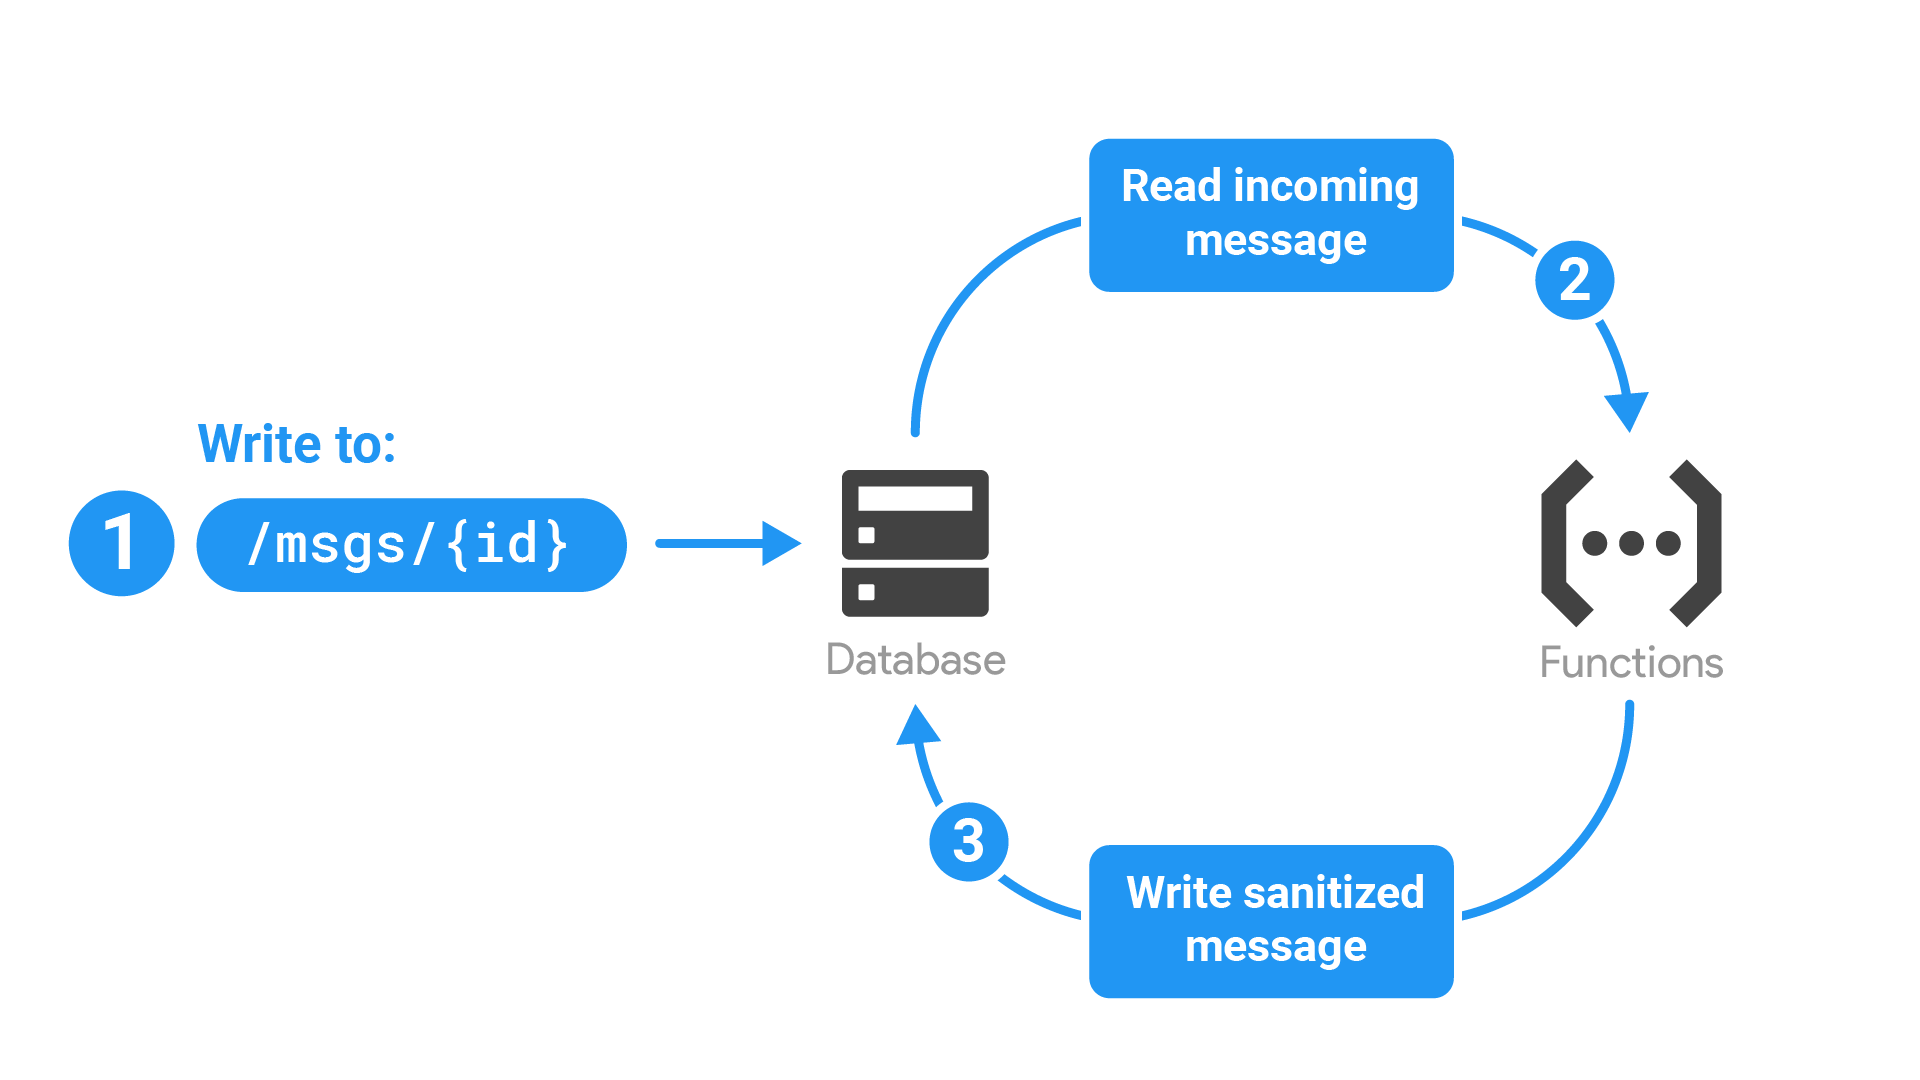
\includegraphics[width=0.3\textwidth]{immagini/functions_ex2.png}
  \caption{Firebase Storage e Cloud Functions esempio 2}
  \label{fig:Firebase Storage e Cloud Functions esempio 2}
\end{figure}

Quando un messaggio viene scritto all'interno della collection "msgs" la funzione che ascolta gli eventi di scrittura ne recupera i dati, elabora il testo per rilevare la presenza di un linguaggio non appropriato e riscrivere il messaggio ricevuto correggendolo o eliminando parti di linguaggio volare, applicando cosi una moderazione del testo lato server.

%https://developer.xamarin.com/guides/android/data-and-cloud-services/google-messaging/firebase-cloud-messaging/
\section{Cloud Messaging}                 %crea la sezione
Firebase Cloud Messaging (FCM) \'e una soluzione di messaggistica multipiattaforma che consente di inviare messaggi tra dispositivi con la possibilt\'a di notificare a una o pi\'u applicazioni client che sono disponibili nuovi dati di sincronizzazione.\\

I messaggi si differenziano in due tipi:
\begin{itemize}
  \item Messaggi di notifica
  \item Messaggi di dati

\end{itemize}

\'E possibile inviare messaggi tramite l'Admin SDK o le API HTTP e XMPP, il carico utile massimo per entrambi i tipi di messaggio \'e 4KB, tranne quando si inviano messaggi dalla console Firebase, che impone un limite di 1024 caratteri.\\
La differenza fra i due tipi di messaggi \'e la loro composizione: i messaggi di notifica contengono un set predefinito di chiavi visualizzabili dall' utente, mentre i messaggi di dati, contengono solo le coppie di valori definite dall'utente.\\
Entrambi i messaggi richiedono di definire il campo obbligatorio "token" che \'e un riferimento ad dispositivo o ad un gruppo di dispositivi, questo token \'e generato tramite l'SDK di Firebase e deve essere memorizzato su un server per poter essere riutilizzato, in caso contrario l'SDK permette di aggiornare il token del dispositivo.\\

\subsection{Invio messaggi}
Firebase Cloud Messaging \'e usufruibile solo se si utilizza l'apposito SDK e si ottiene un token, necessario per inviare un messaggio a un dispositivo specifico.\\
All'avvio iniziale dell' applicazione, l'SDK FCM genera un token di registrazione per l'istanza dell' applicazione client.\\
I token e la ricezione dei messaggi possono essere controllati creando una classe che ha come estensione la classe "FirebaseInstanceIdService" per la gestione dei token e la classe "FirebaseMessagingService" per la gestione dei messaggi ricevuti.\\

Il token di registrazione pu\'o cambiare quando:

\begin{itemize}
    \item L' applicazione elimina l' ID istanza
    \item L' applicazione viene ripristinata su un nuovo dispositivo
    \item L' utente disinstalla/riinstalla l' app
    \item L' utente cancella i dati delle app.
\end{itemize}

FCM tramite l'SDK e richieste HTTPS consente anche la creazione di gruppi di utenti, permettendo con un solo token di inviare un singolo messaggio a pi\'u istanze di un' applicazione in esecuzione su dispositivi appartenenti a un gruppo. Tutti i dispositivi di un gruppo condividono una comune chiave di notifica, che \'e il token utilizzato da FCM per inviare i messaggi a tutti i dispositivi del gruppo. \\

Sulla base del modello di pubblicazione/iscrizione invece, FCM consente di inviare un messaggio a pi\'u dispositivi che hanno si sono registrati ad un particolare argomento.\\
Le applicazioni client possono iscriversi a qualsiasi argomento esistente o creare un nuovo argomento. Quando un' applicazione client sottoscrive un nuovo nome di argomento (uno che non esiste gi\'a per il vostro progetto Firebase), un nuovo argomento di tale nome viene creato in FCM e ogni cliente pu\'o successivamente sottoscriverlo.\\
Per iscriversi a un argomento, l' applicazione client chiama la funzione

\begin{lstlisting}[language=java,caption={FCM topic}]
 FirebaseMessaging.getInstance().subscribeToTopic("news");
\end{lstlisting}

Per annullare l' iscrizione, l' applicazione client deve richiamare unsubscribeFromTopic () con il nome dell' argomento.





\subsection{Parametri}

Oltre al destinatario \'e possobile definire anche la priorit\'a di un messaggio, la durata, il suono, l'icona, il tempo di vita e altri parametri opzionali.

I principali parametri messi a disposizione da Firebase sono:

\begin{table}[h]
\begin{center}
\begin{tabular}{|p{3cm}|p{11cm}|}
\hline
\textbf{Paramentro} & \textbf{Descrizione} \\ \hline
Title &	Titolo della notifica. \\   \hline
Body &	Testo della notifica \\   \hline
Sound  &	Suono da riprodurre quando il dispositivo riceve la notifica. \\   \hline
Sottotitolo  &	Sottotitolo della notifica. \\   \hline
Icon & Icona della notifica \\   \hline
Timetolive & Specifica per quanto tempo (in secondi) il messaggio deve essere conservato se il dispositivo \'e offline.  \\   \hline
Clickaction &	L' azione associata ad un click  della notifica. \\   \hline

\end{tabular}
\caption[Cloud Messaging paramentri ]{FCM parametri}\label{tab:FCFM parametri}
\end{center}
\end{table}


\subsection{Priorit\'a}
Esistono due opzioni per assegnare la priorit\'a di consegna ai messaggi: normale e ad alta priorit\'a. Il recapito di messaggi normali e ad alta priorit\'a funziona in questo modo:
\begin{itemize}
\item Priorit\'a normale: i messaggi vengono inviati immediatamente quando l' app \'e in primo piano, quando invece il dispositivo \'e in modalit\'a Doze o l' applicazione \'e in standby app la consegna potrebbe essere ritardata per risparmiare la batteria, i messaggi in questo caso richiedono di pianificare un job FJD (Firebase Job Dispache) o un JobIntentService per gestire la notifica quando la rete sar\'a nuovamaente disponibile.
\item Alta priorit\'a: Il server Cloud Messaging tenta di inviare immediatamente il messaggio ad alta priorit\'a, consentendo al servizio di attivare un dispositivo sleeping, tramite l'SDK, e di eseguire alcune elaborazioni limitate (compreso un accesso alla rete molto limitato).
\end{itemize}









\section{FirebaseUI}                 %crea la sezione
FirebaseUI \'e un insieme di librerie open-source per Firebase che consentono di semplificare lo sviluppo di un applicaione che utilizza Firebase.
I miglioramenti vengono apportati attraverso una versione semplificata dell' autenticazione di Firebase fornendo metodi di facile utilizzo che si integrano con i pi\'u comuni fornitori di identit\'a come Facebook, Twitter e Google, migliorare la gestone delle view con la sincronizzazione in tempo reale del database e funzionalit\'a aggiuntive per il servizio Firebase Storage

FirebaseUI dispone di moduli separati per utilizzare Firebase Realtime Database, Cloud Firestore, Firebase Auth e Cloud Storage.
\begin{itemize}
  \item FirebaseUI Autorizzare
  \item  FirebaseUIUI Firebase Firestore
  \item  FirebaseUI Database
  \item  FirebaseUI storage
\end{itemize}


FirebaseUI-Auth mira a massimizzare l'integrqzione integra con Smart Lock for Password per memorizzare e recuperare le credenziali, consentendo l' accesso automatico e single-tap sign-in, gestendo anche casi d'uso pi\'u complessi come il recupero dell'account e il collegamento di account multipli che sono sensibili alla sicurezza e difficili da implementare correttamente utilizzando le API di base fornite da Firebase Auth.

FirebaseUI-Firestore semplifica il collegamento dei dati da Cloud Firestore all' interfaccia utente dell' applicazione, fornendo un adapter personalizzato per Firestore (FirestoreRecyclerAdapter) che consente la manipolazione automatica della sincronizzazione tra view e il database Firestore.

\clearpage{\pagestyle{empty}\cleardoublepage}
